\documentclass{beamer}
\beamertemplatenavigationsymbolsempty
\usepackage[french]{babel}
\usepackage{fontspec}
\usepackage{amsmath, amsthm, amsfonts}
\usepackage[separate-uncertainty]{siunitx}
\usepackage{xcolor}
\usepackage{tikz}
\usepackage{tikz-cd}
\usepackage[object=vectorian]{pgfornament}
\usepackage{circuitikz}
\usepackage{hyperref}
\usepackage{caption}
\usepackage{booktabs}
\usepackage{mathtools}
\usepackage{longtable}
\usepackage[version=3]{mhchem}
\usepackage{marginnote}
\usepackage[framemethod=tikz]{mdframed}


% Paul Tol's qualitative palette
% ``bright''.https://personal.sron.nl/~pault/#sec:qualitative
\definecolor{tblue}{HTML}{4477AA}
\definecolor{tcyan}{HTML}{66CCEE}
\definecolor{tgreen}{HTML}{228833}
\definecolor{tyellow}{HTML}{CCBB44}
\definecolor{tred}{HTML}{EE6677}
\definecolor{tpurple}{HTML}{AA3377}
\definecolor{tgrey}{HTML}{BBBBBB}


% Justification for marginnotes.
\renewcommand*{\raggedleftmarginnote}{}
\renewcommand*{\raggedrightmarginnote}{}


% Styles for mdframed environments.
\newmdenv[backgroundcolor=tgreen!10,linecolor=tgreen!30]{reponsebox}
\newmdenv[backgroundcolor=tyellow!10,linecolor=tyellow!30]{diapobox}
\newmdenv[backgroundcolor=tred!10,linecolor=tred!30]{fondamentalbox}

% Default arrow for tikz and style for positive and negative objects.
\tikzset{>=latex,
    negative/.style={draw=teal!70!black, fill=teal!10, thick},
    positive/.style={draw=red, fill=red!10, thick}}
\usetikzlibrary{matrix,calc,decorations.pathreplacing,decorations.pathmorphing,decorations.markings}

% French locale for numbers and negative exponent for units.
\sisetup{locale=FR, per-mode=symbol}

\newcommand{\abs}[1]{\left| #1 \right|}
\newcommand{\rhat}{\vec{\hat{r}}}
\newcommand{\xhat}{\vec{\imath}}
\newcommand{\yhat}{\vec{\jmath}}
\newcommand{\zhat}{\vec{k}}
\newcommand{\real}{\mathbb{R}}
\newcommand{\der}[2]{\frac{\mathrm{d}#1}{\mathrm{d}#2}}
\newcommand{\pder}[2]{\frac{\partial\ #1}{\partial\ #2}}
\newcommand{\dif}{\mathrm{d}}
\newcommand{\ddif}{\,\mathrm{d}}
\newcommand{\grad}{\vec{\nabla}}
\newcommand{\exemple}[1]{\begin{fullwidth}#1\end{fullwidth}}
\newcommand{\norm}[1]{\lVert\ #1\ \rVert}
\newcommand{\vu}{\vec{u}}
\newcommand{\vv}{\vec{v}}
\newcommand{\vr}{\vec{r}}
\newcommand{\va}{\vec{a}}
\newcommand{\vF}{\vec{F}}
\newcommand{\vE}{\vec{E}}
\newcommand{\vB}{\vec{B}}
\newcommand{\vecxyz}[3]{#1 \xhat\ + #2 \yhat\ + #3 \zhat}
\newcommand{\vecxy}[2]{#1 \xhat\ + #2 \yhat}
\newcommand{\coulombcst}{k}
\newcommand{\emf}{\ensuremath{\mathcal{E}}}
\newcommand{\eval}{\SI{1.602e-19}{C}}
\newcommand{\kval}{\SI{8.99e9}{Nm^2 \per C^2}}

% Nice separator line
\newcommand{\sectionline}{
    \noindent
    \begin{center}
        \resizebox{0.5\linewidth}{1ex}
    {{%
    {\begin{tikzpicture}
    \node  (C) at (0,0) {};
    \node (D) at (9,0) {};
    \path (C) to [ornament=85] (D);
    \end{tikzpicture}}}}
    \end{center}
}

\theoremstyle{definition}
\newtheorem*{defn}{Definition}


\usepackage[version=3]{mhchem}

\setbeamercolor{title}{fg=tblue}
\setbeamercolor{frametitle}{fg=tblue}
\setbeamercolor{structure}{fg=tblue}

% Make footnotesize smaller
\makeatletter
\renewcommand\footnotesize{%
   \@setfontsize\footnotesize\@viipt{11}%
   \abovedisplayskip 8\p@ \@plus2\p@ \@minus4\p@
   \abovedisplayshortskip \z@ \@plus\p@
   \belowdisplayshortskip 4\p@ \@plus2\p@ \@minus2\p@
   \def\@listi{\leftmargin\leftmargini
               \topsep 4\p@ \@plus2\p@ \@minus2\p@
               \parsep 2\p@ \@plus\p@ \@minus\p@
               \itemsep \parsep}%
   \belowdisplayskip \abovedisplayskip
}
\makeatother

\title{Électricité et magnétisme}
\subtitle{Chapitre 10 - Induction électromagnétique}
\date{30 novembre 2021}
\author{Loïc Séguin-Charbonneau}
\institute{Cégep Édouard-Montpetit}

\begin{document}

\maketitle

\begin{frame}{Fluide}
  Un fluide s'écoule à travers une boucle. Dans laquelle des situations la
  quantité de fluide qui traverse la boucle est-elle la plus grande?

  \begin{center}
    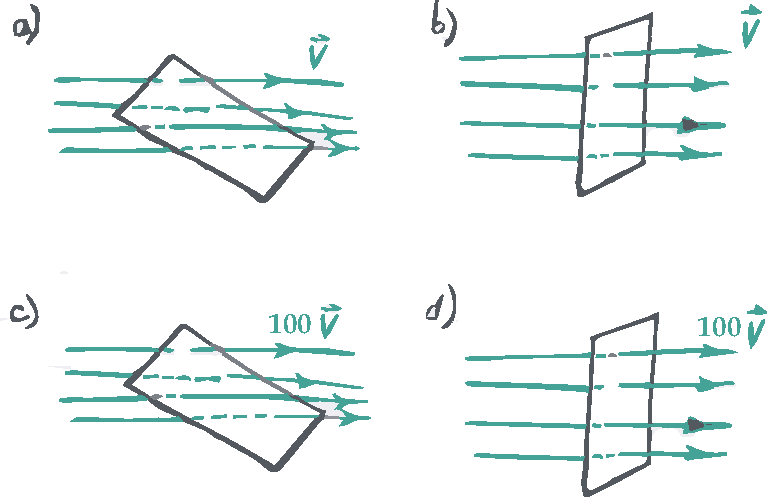
\includegraphics[scale=0.8]{figures/flux.pdf}
  \end{center}
\end{frame}


\begin{frame}{Flux magnétique}
  La boucle ci-contre est dans une région où se trouve un champ magnétique
  uniforme $\vB = \left(\vecxyz{1}{1}{1}\right) \si{G}$. Quel est le flux
  magnétique à travers la boucle?
    \begin{center}
      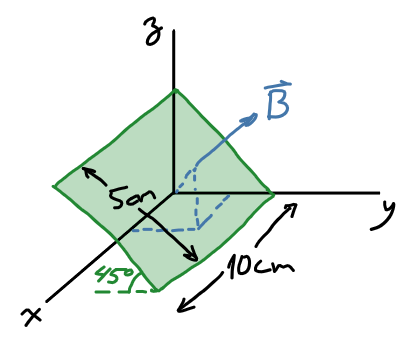
\includegraphics[width=5cm]{figures/flux-boucle-1.png}
    \end{center}
\end{frame}


\begin{frame}[t]{Loi de Lenz}
  Une boucle de fil se trouve dans un champ magnétique uniforme tel qu'illustré
  sur le dessin ci-dessous.

  \only<1-4>{
    \begin{center}
      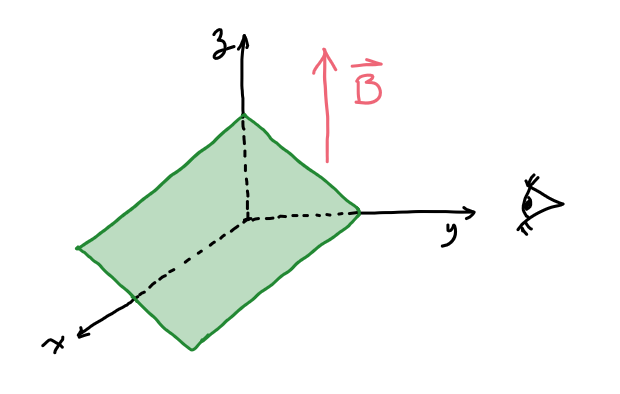
\includegraphics[width=5cm]{figures/boucle_oeil.png}
    \end{center}
  }

  \only<5-6>{
    \begin{center}
      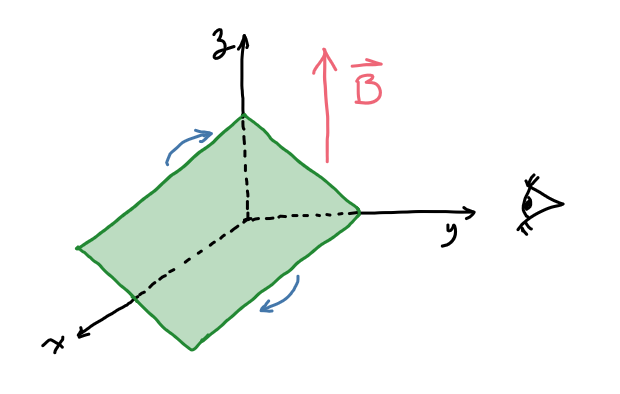
\includegraphics[width=5cm]{figures/boucle_oeil_tourne.png}
    \end{center}
  }

  \only<1-2>{
    La grandeur du champ magnétique augmente avec le temps. Quelle est la
    direction du courant induit dans la boucle?

    \begin{enumerate}[A.]
      \item<alert@2> sens horaire
      \item sens anti-horaire
      \item aucun courant induit
    \end{enumerate}

  }

  \only<3-4>{
    La grandeur du champ magnétique diminue avec le temps. Quelle est la
    direction du courant induit dans la boucle?

    \begin{enumerate}[A.]
      \item sens horaire
      \item<alert@4> sens anti-horaire
      \item aucun courant induit
    \end{enumerate}

  }

  \only<5-6>{
    La boucle tourne dans le sens indiqué sur le dessin. Quelle est la direction
    du courant induit dans la boucle?

    \begin{enumerate}[A.]
      \item sens horaire
      \item<alert@6> sens anti-horaire
      \item aucun courant induit
    \end{enumerate}

  }

\end{frame}


\begin{frame}[t]{Loi de Faraday - Champ magnétique variable}
  Une bobine circulaire de \SI{5}{\centi\meter} de rayon comportant \num{50}
  tours se trouve dans un champ magnétique uniforme dont la grandeur varie dans
  le temps tel qu'illustré dans le graphique ci-dessous.
  \begin{center}
    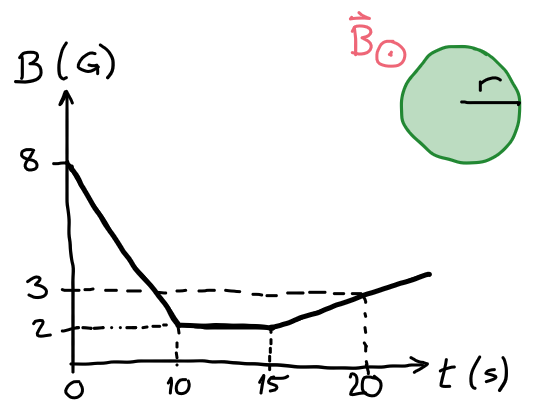
\includegraphics[width=5cm]{figures/champ_variable.png}
  \end{center}

  Déterminez la f.é.m. induite et la direction du courant à
  \begin{enumerate}
    \item $t = \SI{5}{\second}$
              \only<2>{
                \alert{
                  \,\,\SI{0.2356e-4}{\volt},
                  courant dans le sens anti-horaire
                }
              }
    \item $t = \SI{11}{\second}$
               \only<2>{\alert{\,\,\SI{0}{\volt}}}
    \item $t = \SI{20}{\second}$
               \only<2>{
                 \alert{
                   \,\,\SI{0.0785e-4}{\volt}, courant dans le sens horaire
                 }
               }
  \end{enumerate}
\end{frame}


\begin{frame}[t]{Générateur linéaire}

  Un cadre métallique fixe sert de support à une tige métallique mobile. La tige
  se déplace vers la droite à \SI{20}{cm/s} et sa longueur est de \SI{35}{cm}. Le
  champ magnétique externe est uniforme de \SI{120}{G}.
  Si la résistance de la boucle est de \SI{4}{\ohm}, déterminer le courant induit
  dans la boucle.

  \begin{center}
  \begin{tikzpicture}[>=latex]
    \draw[thick] (5, 0) -- (0, 0) -- (0, 3) -- (5, 3);
    \draw[thick, fill] (2, -0.15) rectangle (2.15, 3.15);
    \draw[->] (2.25, 1.5) -- ++(1, 0) node[right] {$\vec{v}$};
    \draw[|<->|] (-0.4, 0) -- node[fill=white] {$L$} (-0.4, 3);
    \draw (3, 3.5) circle (0.15);
    \draw (2.894, 3.394) -- (3.1061, 3.6061);
    \draw (2.894, 3.6061) -- (3.1061, 3.394);
    \node at (3.3, 3.8) {$\vec{B}$};
  \end{tikzpicture}
  \end{center}
  \only<2>{\alert{\SI{0.210}{\milli\ampere}, courant anti-horaire}}
\end{frame}

\end{document}
